\chapter{はじめに}

\section{研究の背景}
当研究室では例年,高専ロボコンに出場するためのロボットの設計・製作を行っている.今年度はプラスティック製段ボールを如何に高く積み上げるかを競うための積込ロボットの製作を行った.この積み込みロボットにはリフトが搭載されており(図\ref{fig:robot}),このリフトが上下することでプラスティック製段ボールの箱を持ち上げたり降ろすことが出来る.リフトには上端と下端にリミットセンサが設置されており,その位置でリフトが停止するようになっている.しかし,リミットセンサによる位置検出では,センサのある場所にしかリフトを停止させることが出来ない.任意の高さで停止させるには位置を連続的に検出できるセンサを使用した位置制御が必要になるが,そのようなセンサの使用にはコストがかかる.そこで,コストのかかるセンサを使用せずに位置制御を行う方法はないかと考えた.

\begin{figure}[htbp]
  \begin{center}
    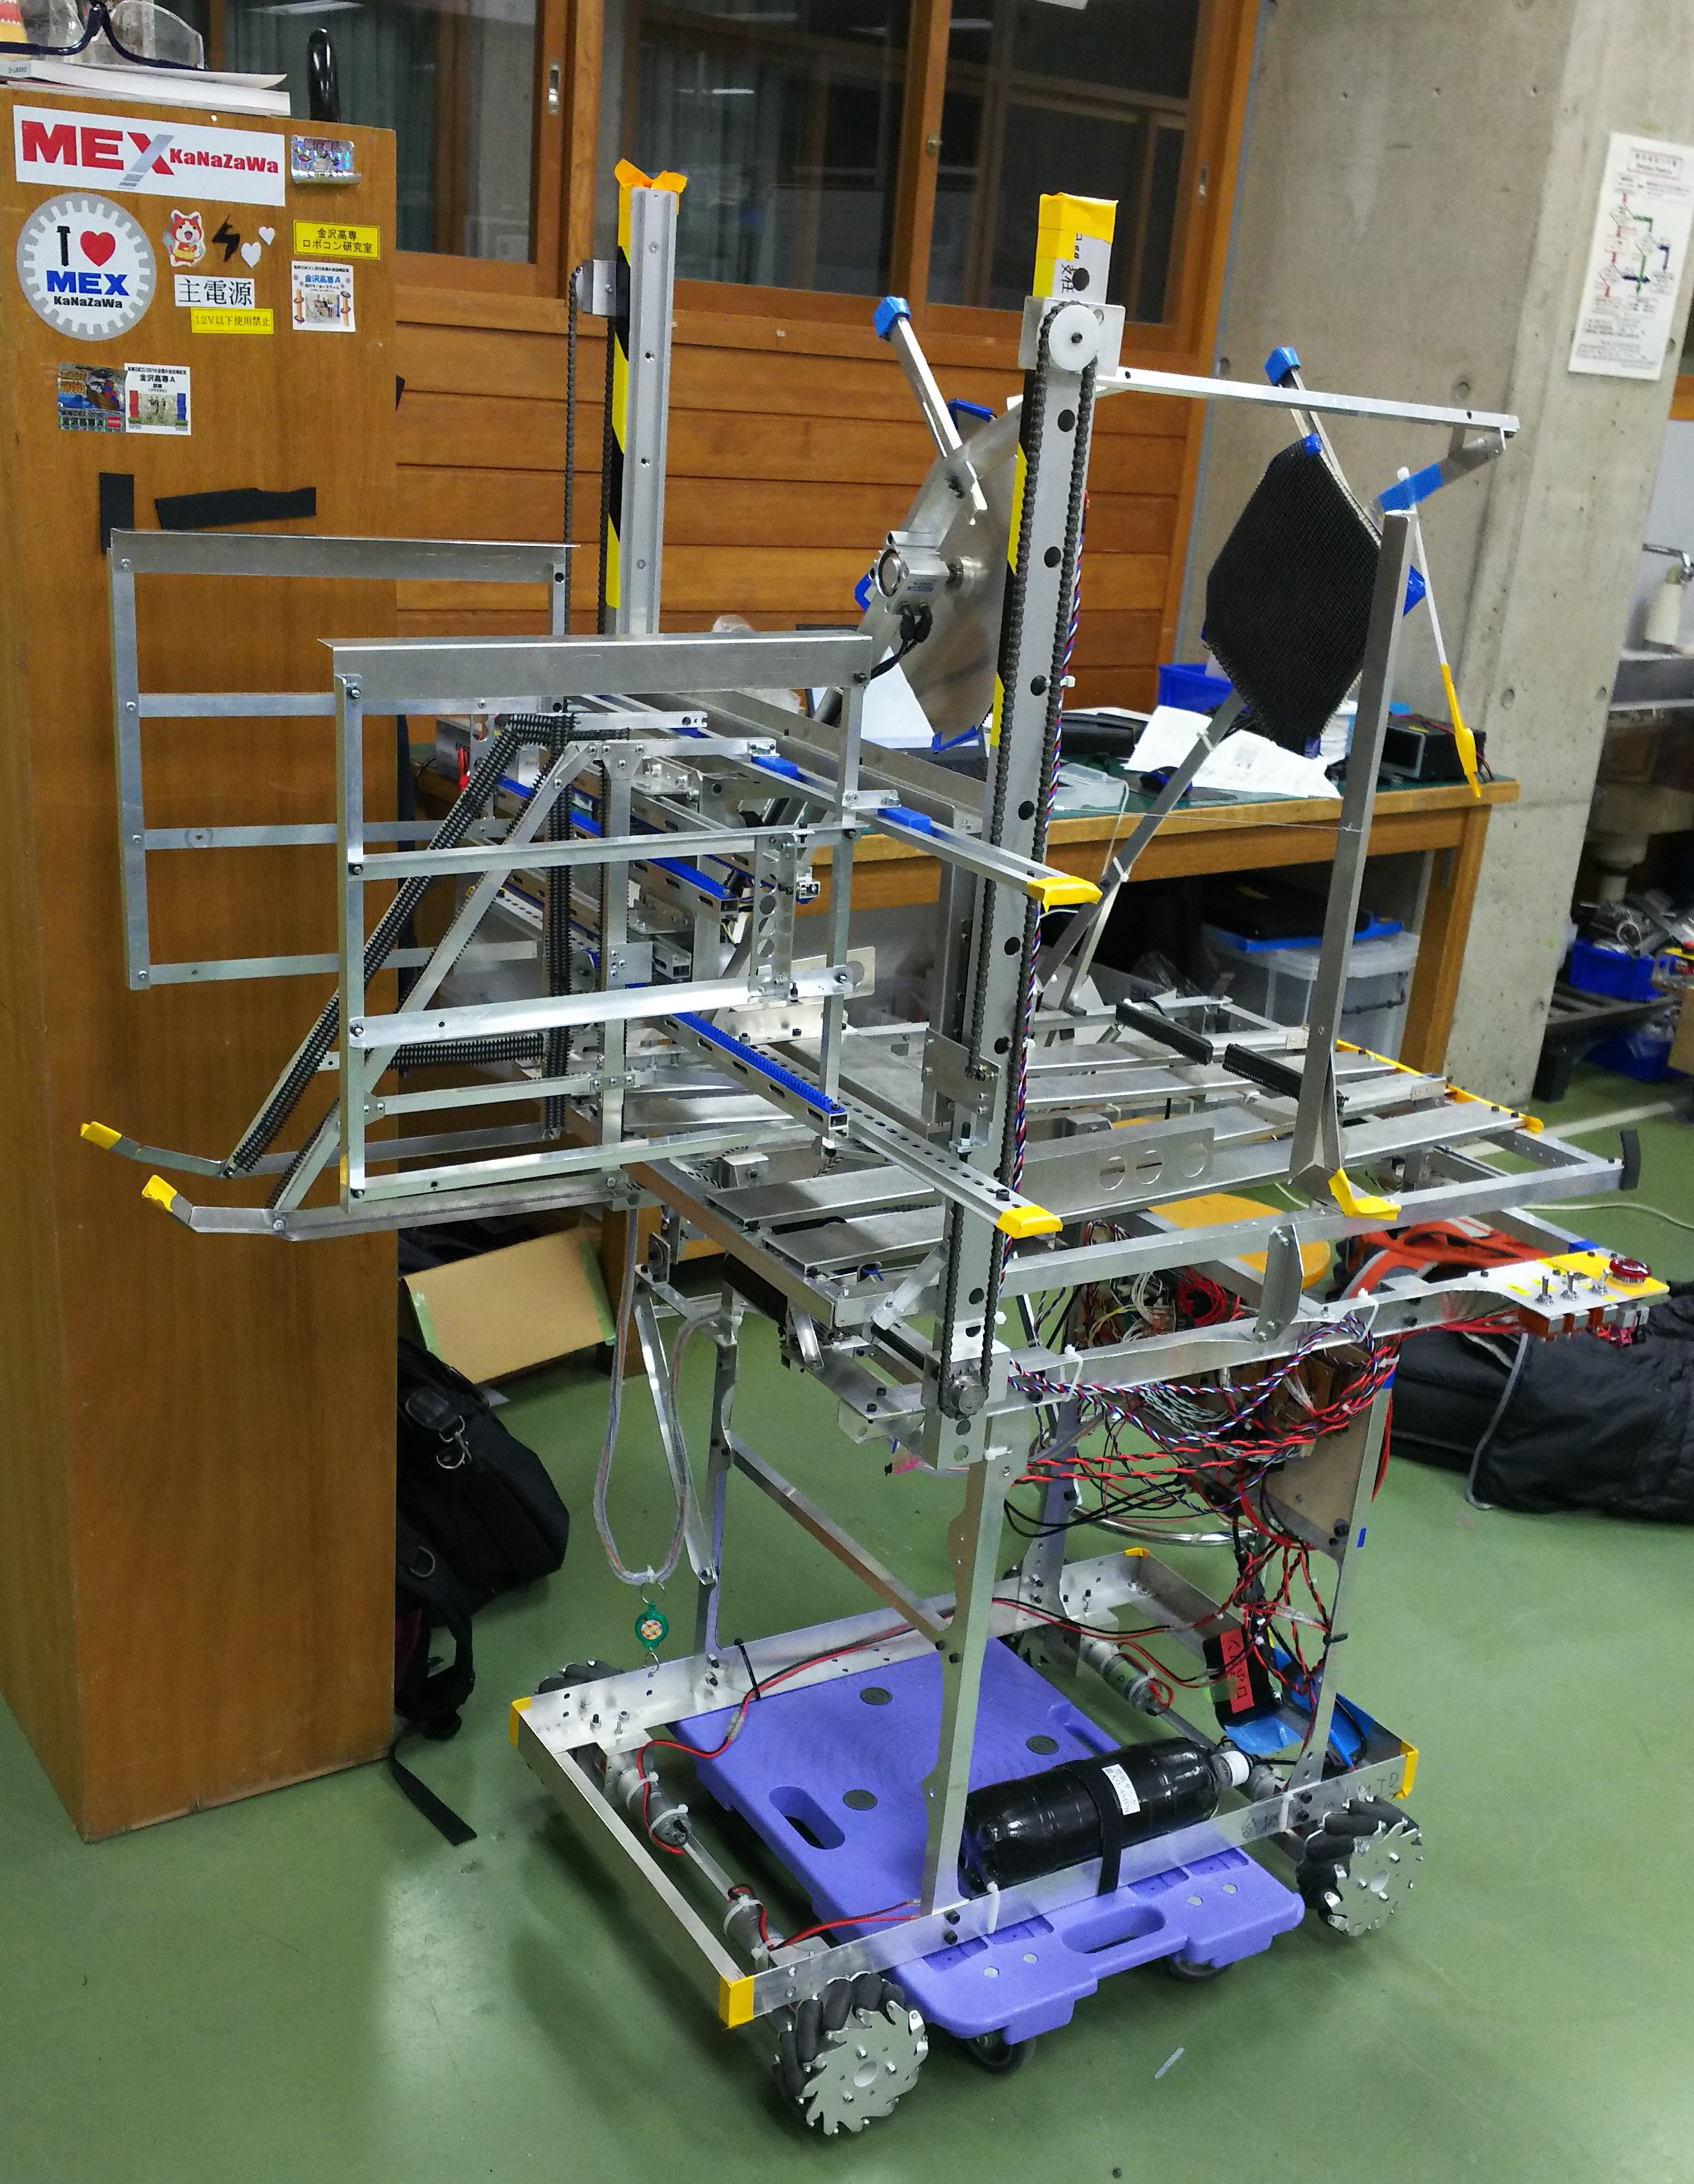
\includegraphics[width=80mm]{img/robot.JPG}
    \end{center}
  \caption{積み込みロボット}
 \label{fig:robot}
\end{figure}

\section{研究の目的}
リミットセンサによる位置検出システムは,走行中の段差などの衝撃によってプラスティック製段ボールの支持位置が変わった際,積み上げ時に繊細な高さ調整が困難であった.さらに,積み上げ時に落下させた場合積み込み幅が大きく変わってしまい積み上げの精度が悪くなる恐れがあった.センサーレス位置検出システムでは任意の高さでの停止が可能になるため,積み上げ時の段ボールの落下による積み込み幅の変動が無くなるのではないかと考えた.このことからロータリーエンコーダやポテンショメータといった,直接リフトの位置を検出できるセンサを使用することなく,リフトを任意の位置に停止させる制御を考案しようと考えた.


\section{本論文の構成}
1章では,本研究の背景と簡略化した概要を示す.2章では製作したリフトについて,高専ロボコンのルールをからめつつ述べる.3章では通常用いられる位置制御について述べる.4章では位置センサを使用しない制御の手法について述べる.5章ではシミュレーションソフトを用いた実験を示す.6章で最後に本実験のまとめを述べる.